\section{Horizontal excess and baseline cancellation}
We bound lower priority-band failures and quantile movement together.
Let $h:[0,1]\to[0,1]$ be nondecreasing and measurable, let $u=h(0)$, and let
$\beta$ and $\zeta$ be as defined in Section~\ref{sec:meta-scalar}.
Define the baseline $q(x)=\max\{u,x\}$. The scalar area bound gives
$\int_0^1(h(x)-q(x))_+\,dx\le\zeta$.
Use the band parameters from \eqref{eq:meta-band-domain}.
Let $\mathcal A$ be the \emph{failure set} of $\alpha\in[\ell,1]$ with
$\alpha>u$ and $h(\alpha-\kappa)\ge\alpha$. Define the \emph{excess region}
and two subregions by
\begin{align*}
 \mathcal E&=\{(x,y):0\le x\le1,\ \max\{u,x\}<y\le h(x)\},\\
 \mathcal H&=\{(x,y):y\in\mathcal A,\ y-\kappa<x<y\},\\
 \mathcal R&=\mathcal E\cap\{1-\kappa<x<1\}.
\end{align*}
If $\mathcal A$ is nonempty, put $v=\inf\mathcal A$ and define the
\emph{clipped triangle}
\[
 \mathcal T=\{(x,y):v-\kappa<x<v,\ \max\{u,x\}<y<v\}.
\]
\begin{figure}[htbp]
\centering
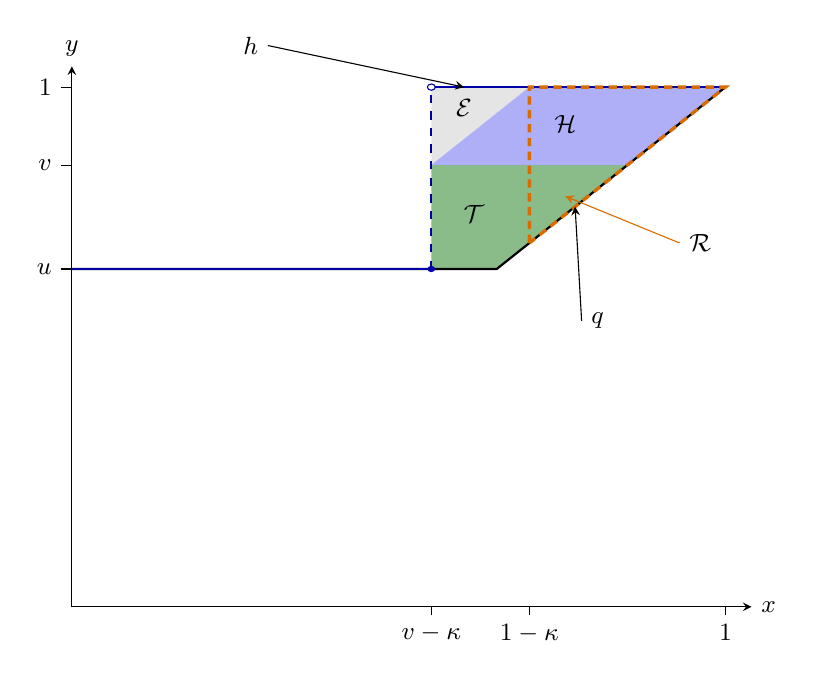
\begin{tikzpicture}[x=8.3cm,y=6.6cm,>=stealth,font=\small]
  \fill[black!10] (.55,.65)--(.55,1)--(1,1)--(.65,.65)--cycle;
  \fill[blue!40,opacity=.70] (.55,.85)--(.85,.85)--(1,1)--(.7,1)--cycle;
  \fill[green!50!black,opacity=.40] (.55,.65)--(.65,.65)--(.85,.85)--(.55,.85)--cycle;
  \draw[->] (0,0)--(1.04,0) node[right] {$x$};
  \draw[->] (0,0)--(0,1.04) node[above] {$y$};
  \draw[thick] (0,.65)--(.65,.65)--(1,1);
  \draw[thick,blue!65!black] (0,.65)--(.55,.65);
  \draw[thick,dashed,blue!65!black] (.55,.65)--(.55,1);
  \draw[thick,blue!65!black] (.55,1)--(1,1);
  \fill[blue!65!black] (.55,.65) circle[radius=.006];
  \filldraw[fill=white,draw=blue!65!black] (.55,1) circle[radius=.006];
  \draw[very thick,densely dashed,orange!85!black] (.7,.7)--(.7,1)--(1,1)--cycle;
  \draw (.55,0)--(.55,-.016) node[below] {$v-\kappa$};
  \draw (.7,0)--(.7,-.016) node[below] {$1-\kappa$};
  \draw (1,0)--(1,-.016) node[below] {$1$};
  \draw (0,.65)--(-.016,.65) node[left] {$u$};
  \draw (0,.85)--(-.016,.85) node[left] {$v$};
  \draw (0,1)--(-.016,1) node[left] {$1$};
  \node at (.615,.755) {$\mathcal T$};
  \node at (.755,.93) {$\mathcal H$};
  \node at (.6,.96) {$\mathcal E$};
  \draw[->,orange!85!black] (.93,.70) node[right,black] {$\mathcal R$} -- (.755,.79);
  \draw[->] (.3,1.08) node[left] {$h$} -- (.6,1);
  \draw[->] (.78,.55) node[right] {$q$} -- (.77,.77);
\end{tikzpicture}
\caption{An example with $\kappa=0.3$, $\ell=0.7$, and $u=0.65$.
The function $h$ equals $0.65$ at and before its jump at $0.55$ and equals $1$
after the jump. The dashed segment marks the jump, and the open and filled
points specify its value there. The
grey background together with the blue and green regions is $\mathcal E$.
The blue region is $\mathcal H$, and the green clipped triangle is
$\mathcal T$, where the infimum of the failure levels is
$v=0.85$. Region shading ignores boundary points. The orange outline marks
$\mathcal R$. In this example its
intersections with $\mathcal H$ and $\mathcal T$ partition $\mathcal R$
up to boundary points, so their combined area attains $\kappa^2/2$.}
\label{fig:excess-regions}
\end{figure}

Figure~\ref{fig:excess-regions} illustrates the construction.

\begin{lemma}[Excess-area accounting]
\label{lem:geometric-overlap}
If $u\le\ell$, then
\[
 |\mathcal A|+|\mathcal R|
 \le \frac{\zeta}{\kappa}
 +\max\left\{0,\frac{\kappa^2}{2}
                  -\frac{\kappa^2-(u-\ell+\kappa)_+^2}{2\cdot\kappa}\right\}.
\]
\end{lemma}
\begin{proof}
Monotonicity gives $h(x)\ge h(y-\kappa)\ge y$ for $(x,y)\in\mathcal H$.
Since $y>\max\{u,x\}$, we have $\mathcal H\subseteq\mathcal E$,
$|\mathcal H|=\kappa\cdot|\mathcal A|$, and $|\mathcal E|\le\zeta$.
If $|\mathcal A|=0$, then $|\mathcal R|\le\zeta\le\zeta/\kappa$.

Otherwise, $v\ge\max\{u,\ell\}$. For $v-\kappa<x<v$, choose
$\alpha\in\mathcal A$ with $\alpha<x+\kappa$. Monotonicity gives
$h(x)\ge h(\alpha-\kappa)\ge\alpha\ge v$.
Consequently $\mathcal T$ lies in $\mathcal E$ and is disjoint from
$\mathcal H$, whose points have second coordinate at least $v$. Its area is
\[
 |\mathcal T|=\frac{\kappa^2-(\kappa-v+u)_+^2}{2},
\]
since the excluded part below $y=u$ is a triangle with side length
$(\kappa-v+u)_+$. As $v\ge\ell\ge u$, this side length is at most
$(u-\ell+\kappa)_+\le\kappa$. Hence
\[
 |\mathcal T|\ge
 \frac{\kappa^2-(u-\ell+\kappa)_+^2}{2}.
\]
The sets $\mathcal H$ and $\mathcal T$ are disjoint subsets of
$\mathcal E$. Also $\mathcal R\subseteq\mathcal E$ and $\kappa\le1$.
Splitting $\mathcal R$ according to these two sets therefore gives
\[
\begin{aligned}
 \kappa\cdot|\mathcal A|+|\mathcal T|+\kappa\cdot|\mathcal R|
 &=|\mathcal H|+|\mathcal T|
   +\kappa\cdot|\mathcal R\setminus(\mathcal H\cup\mathcal T)|\\
 &\quad +\kappa\cdot|\mathcal R\cap(\mathcal H\cup\mathcal T)|\\
 &\le|\mathcal E|+\kappa\cdot
   \underbrace{|\mathcal R\cap(\mathcal H\cup\mathcal T)|}_{\le\,\kappa^2/2}
 \le\zeta+\frac{\kappa^3}{2}.
\end{aligned}
\]
The underbraced intersection lies in the triangle
$1-\kappa<x<y\le1$, which has area $\kappa^2/2$. Dividing by $\kappa$
and using the lower bound on $|\mathcal T|$ proves the claim.
\end{proof}

\begin{lemma}[Movement of the ideal baseline]
\label{lem:geometric-baseline}
If $u\le\ell$, then
\[
 \mathcal M(q)=\kappa\cdot(1-\ell)
 -\frac{(u-\ell+\kappa)_+^2}{2}.
\]
\end{lemma}
\begin{proof}
Since $q(x)=x+(u-x)_+$,
\[
 \mathcal M(q)=\kappa\cdot(1-\ell)
 +\int_{1-\kappa}^1(u-x)_+\,dx
 -\int_{\ell-\kappa}^{\ell}(u-x)_+\,dx.
\]
Because $u\le\ell\le1-\kappa$, the first integral vanishes and the
second equals $(u-\ell+\kappa)_+^2/2$.
\end{proof}

\begin{lemma}[Upper-baseline bound]
\label{lem:geometric-hinge}
If $u\ge\ell$, then
\[
 \bigl|\{\alpha\in[\ell,1]:h(\alpha-\kappa)\ge\alpha\}\bigr|
 +\mathcal M(h)
 \le \kappa\cdot(1-\ell)+(1-\kappa)\cdot(u-\ell)
      +\kappa\cdot(1-\beta)+\frac{\zeta}{\kappa}.
\]
\end{lemma}
\begin{proof}
The failure set at levels at most $u$ has measure $u-\ell$, since
$h(\alpha-\kappa)\ge u\ge\alpha$ for $\ell\le\alpha\le u$.
Since $\kappa\le1$ and $\mathcal H\cup\mathcal R\subseteq\mathcal E$,
\[
 \kappa\cdot(|\mathcal A|+|\mathcal R|)
 \le|\mathcal H\cup\mathcal R|+\kappa\cdot|\mathcal H\cap\mathcal R|
 \le\zeta+\kappa\cdot|\mathcal H\cap\mathcal R|.
\]
Dividing by $\kappa$ bounds $|\mathcal A|+|\mathcal R|$.
The intersection lies above $u$, so
\[
 |\mathcal H\cap\mathcal R|
 \le\int_{1-\kappa}^{1}(1-\max\{u,x\})_+\,dx.
\]
Since $q(x)=u+(x-u)_+$ and $q(x)=u$ on $[\ell-\kappa,\ell]$,
\[
 \mathcal M(q)=\int_{1-\kappa}^{1}(x-u)_+\,dx.
\]
The integrands in the last two displays add to $1-u$, as $u\le1$.
Thus $|\mathcal H\cap\mathcal R|+\mathcal M(q)\le\kappa\cdot(1-u)$.
Finally, the last inequality in Lemma~\ref{lem:meta-scalar-area} gives $h(x)\ge q(x)-(1-\beta)$,
and the definition of $\mathcal R$ gives
\[
 \mathcal M(h)\le\mathcal M(q)+\kappa\cdot(1-\beta)+|\mathcal R|.
\]
Adding the bounds and using
$(u-\ell)+\kappa\cdot(1-u)=\kappa\cdot(1-\ell)+(1-\kappa)\cdot(u-\ell)$ proves the claim.
\end{proof}

For $0\le u\le1$ define
\[
 \Gamma(u)=
 \begin{cases}
 0,&u\le\ell-\kappa,\\
 \max\left\{-\dfrac{(u-\ell+\kappa)^2}{2},
 -\dfrac{\ell-u}{4}\right\},
       &\ell-\kappa\le u\le\ell,\\
 (1-\kappa)\cdot(u-\ell),&u\ge\ell.
 \end{cases}
\]
The formulas agree at the two shared endpoints.

\begin{corollary}[Combined failure and movement bound]
\label{cor:meta-negative-well}
We have
\[
 \bigl|\{\alpha\in[\ell,1]:h(\alpha-\kappa)\ge\alpha\}\bigr|
 +\mathcal M(h)
 \le\kappa\cdot(1-\ell)+\Gamma(u)+\kappa\cdot(1-\beta)+\zeta/\kappa.
\]
\end{corollary}
\begin{proof}
For $u\ge\ell$, Lemma~\ref{lem:geometric-hinge} gives the claim.
For $u\le\ell$, the failure set has measure $|\mathcal A|$. The scalar
crossing bound and the definition of $\mathcal R$ give
\[
 \mathcal M(h)\le\int_{1-\kappa}^{1}q(x)\,dx
 -\int_{\ell-\kappa}^{\ell}q(x)\,dx
 +\kappa\cdot(1-\beta)+|\mathcal R|.
\]
By Lemmas~\ref{lem:geometric-overlap} and~\ref{lem:geometric-baseline},
the failure measure plus the movement is at most
\[
 \kappa\cdot(1-\ell)+\kappa\cdot(1-\beta)+\frac{\zeta}{\kappa}
 +\max\left\{-\frac{(u-\ell+\kappa)_+^2}{2},
   \left(1-\frac1\kappa\right)\cdot
   \frac{\kappa^2-(u-\ell+\kappa)_+^2}{2}\right\}.
\]
The maximum is zero if $u\le\ell-\kappa$. For
$\ell-\kappa\le u\le\ell$, its second branch is
\[
 - (1-\kappa)\cdot(\ell-u)\cdot
 \left(1-\frac{\ell-u}{2\cdot\kappa}\right)
 \le-\frac{\ell-u}{4},
\]
because $0\le\ell-u\le\kappa\le1/2$. The resulting bound is
$\Gamma(u)$.
\end{proof}
\section{Joint scalar charges and the signed moment}
\label{sec:meta-joint}

Use the parameters in Appendix~\ref{sec:meta-parameters}.
The scalar charges and coefficient collection below also apply to any real
parameters satisfying the band conditions and inequalities stated below.
The final numerical step uses the particular choice in the appendix.
The appendix verifies the band conditions and the following two inequalities:
\begin{equation}
 (1-\ell)\cdot(u-U)_++\Gamma(u)
 \le\frac{Q\cdot (c+2)}{2}\cdot(u-c)^2+\lambda\cdot(u-c)+\nu
 \qquad(0\le u\le1)
 \label{eq:meta-majorant}
\end{equation}
and
\begin{equation}
 1+\kappa\cdot(2-\ell)\le\frac{Q\cdot(1-c)}2+\lambda\cdot c-\nu.
 \label{eq:meta-defect-domain}
\end{equation}
The parameter values also satisfy $Q>0$ and $\kappa\le1$.
They satisfy $Q\cdot\kappa\ge c$ as well.

\begin{lemma}[Charge when $\beta_i>c$]
\label{lem:meta-good-charge}
For every $i\in\mathcal J$ with $\beta_i>c$,
\begin{equation}
 (1-\ell)\cdot(u_i-U)_++\mathcal F_i+\mathcal M(h_i)
 \le (\kappa\cdot(1-\ell)+\nu)\cdot\beta_i+\lambda\cdot(u_i-c\cdot\beta_i)
       +Q\cdot f_i+\zeta_i/\kappa.
 \label{eq:meta-good-complete}
\end{equation}
\end{lemma}
\begin{proof}
Since $\beta_i>c$, the deficit identity \eqref{eq:meta-f-square} gives
\begin{align*}
 Q\cdot f_i+\lambda\cdot(u_i-c\cdot\beta_i)+\nu\cdot\beta_i
 &=\frac{Q\cdot (c+2)}{2}\cdot(u_i-c)^2+\lambda\cdot(u_i-c)+\nu\\
 &\quad +(1-\beta_i)\cdot
   \left[\frac{Q\cdot (c+2)}{2}\cdot(\beta_i-c^2)+\lambda\cdot c-\nu\right]\\
 &\ge (1-\ell)\cdot(u_i-U)_++\Gamma(u_i)+[1+\kappa\cdot(2-\ell)]\cdot(1-\beta_i).
\end{align*}
The last step uses the majorant \eqref{eq:meta-majorant}, the identity
$(c+2)\cdot(c-c^2)=1-c$, and \eqref{eq:meta-defect-domain}. In particular,
$\beta_i>c$ and $Q>0$ bound the bracket below by
$Q\cdot(1-c)/2+\lambda\cdot c-\nu$.
Corollary~\ref{cor:meta-negative-well}, $\theta_i\le1$, and the upper-failure
bound $1-\beta_i$ give
\[
 \mathcal F_i+\mathcal M(h_i)\le
 \kappa\cdot(1-\ell)+\Gamma(u_i)+(1+\kappa)\cdot(1-\beta_i)+\zeta_i/\kappa.
\]
Writing $\kappa\cdot(1-\ell)$ as
$\kappa\cdot(1-\ell)\cdot\beta_i+\kappa\cdot(1-\ell)\cdot(1-\beta_i)$ proves the claim.
\end{proof}

The appendix also verifies
\begin{equation}
 \frac{1-\ell}{U}\le1+\lambda,\qquad
 1-\kappa\cdot(1-\ell)-\nu+\lambda\cdot c
 \le Q\cdot c.
 \label{eq:meta-low-parameters}
\end{equation}

\begin{lemma}[Deficit bound]
\label{lem:low-crossing-deficit}
If $0\le u\le\beta\le c$, then
\[
 f(u,\beta)\ge c\cdot\beta.
\]
\end{lemma}
\begin{proof}
The difference factors as
\[
 f(u,\beta)-c\cdot\beta
 =(\beta-u)\cdot\left[1-\frac{c+2}{2}\cdot(\beta+u)\right].
\]
Both factors are nonnegative since $u\le\beta\le c$ and
$(c+2)\cdot c=1$.
\end{proof}

\begin{lemma}[Charge when $\beta_i\le c$]
\label{lem:meta-bad-charge}
For every $i\in\mathcal J$ with $\beta_i\le c$,
the bound \eqref{eq:meta-good-complete} holds.
\end{lemma}
\begin{proof}
The shifted-integral representation of $\mathcal M$ and $h_i-u_i\ge0$ give
\[
 \mathcal M(h_i)\le\int_{1-\kappa}^1(h_i(x)-u_i)\,dx
 \le\int_0^1(h_i(x)-u_i)\,dx
 =\zeta_i+u_i^2/2+\beta_i-\beta_i^2/2-u_i.
\]
The total weighted failure is at most
$(1-\ell)\cdot\min\{u_i/U,1\}$, by the pool-weight bound.
Thus the complete cost is at most
\[
 (1-\ell)\cdot[(u_i-U)_++\min\{u_i/U,1\}]
 +u_i^2/2+\beta_i-\beta_i^2/2-u_i+\zeta_i.
\]
For $0\le u\le1$, the hinge terms satisfy
\[
 (u-U)_++\min\{u/U,1\}\le u/U.
\]
This holds with equality for $u\le U$. For $u\ge U$, the difference
between the right and left sides is $(1-U)\cdot(u/U-1)\ge0$.
Using this inequality and $u_i^2\le\beta_i^2$, we obtain
\begin{align*}
 &(1-\ell)\cdot[(u_i-U)_++\min\{u_i/U,1\}]
   +u_i^2/2+\beta_i-\beta_i^2/2-u_i\\
 &\quad-(\kappa\cdot(1-\ell)+\nu)\cdot\beta_i
   -\lambda\cdot(u_i-c\cdot\beta_i)\\
 &\le\left[\frac{1-\ell}{U}-1-\lambda\right]\cdot u_i
   +[1-\kappa\cdot(1-\ell)-\nu+\lambda\cdot c]\cdot\beta_i\\
 &\le Q\cdot c\cdot\beta_i
 \le Q\cdot f_i.
\end{align*}
The last line uses \eqref{eq:meta-low-parameters} and
Lemma~\ref{lem:low-crossing-deficit}. Since $\kappa\le1$ and
$\zeta_i\ge0$, the complete cost is at most the claimed bound.
\end{proof}

\subsection{Eliminating the signed moment}
The following identity follows from the exact-capacity equality and the
scalar gap identity in Section~\ref{sec:meta-pool}:
\begin{equation}
 \frac1m\cdot\sum_{i\in\mathcal J}(u_i-c\cdot\beta_i)
 =(c+1)\cdot M_j(0)-C_j^{\mathrm{LP}}+\tfrac12
 +\frac{c}{m}\cdot\sum_{i\in\mathcal J}\bigl(f_i+(c+2)\cdot\zeta_i\bigr).
 \label{eq:meta-moment-identities}
\end{equation}
Indeed, the left side equals
$M_j(0)-\frac{c}{m}\cdot\sum_{i\in\mathcal J}\beta_i$. Substitute the
identity for the sum of the $\beta_i$ and use $(c+2)\cdot c=1$.

\begin{lemma}[Per-job bound]
\label{thm:meta-symbolic}
For every original target $j$ and every feasible LP solution,
\[
 \mathbb E[\widetilde C_j]\le
 \left(c+2-0.0288468\right)\cdot C_j^{\mathrm{LP}}.
\]
\end{lemma}
\begin{proof}
The gap estimate \eqref{eq:meta-gap-identity} and $I_j(\alpha)\le a_j$ imply
\begin{equation}
 (c+2)\cdot C_j^{\mathrm{LP}}-\mathbb E[\widetilde C_j]
 \ge\frac1m\cdot\sum_{i\in\mathcal J}
       \bigl(f_i+(c+2)\cdot\zeta_i\bigr)
       +M_j(0)-a_j+1+\frac c2.
 \label{eq:meta-base-gap}
\end{equation}
Apply Lemma~\ref{lem:integrated-partial-pool} and, for each job, the applicable
charge from Lemmas~\ref{lem:meta-good-charge} and~\ref{lem:meta-bad-charge}.
Since $Q\cdot\kappa\ge c$ and $(c+2)\cdot c=1$, we have
$\zeta_i/\kappa\le Q\cdot(c+2)\cdot\zeta_i$. Summing over jobs gives
\begin{align*}
 (c+2)\cdot C_j^{\mathrm{LP}}-\mathbb E[\widetilde C_j]
 &\ge \frac1m\cdot\sum_{i\in\mathcal J}\bigl(f_i+(c+2)\cdot\zeta_i\bigr)
       +M_j(0)-a_j+1+\frac c2\\
 &\quad +a_j\cdot(1-\ell)\cdot(1-U)-(1-\ell)\cdot(2-U)\\
 &\quad -\frac{\kappa\cdot(1-\ell)+\nu}{m}\cdot\sum_{i\in\mathcal J}\beta_i
 -\frac{\lambda}{m}\cdot\sum_{i\in\mathcal J}(u_i-c\cdot\beta_i)\\
 &\quad -\frac Qm\cdot\sum_{i\in\mathcal J}\bigl(f_i+(c+2)\cdot\zeta_i\bigr).
\end{align*}
Substitute \eqref{eq:meta-moment-identities} for the signed moment and the
scalar identity for $\sum_{i\in\mathcal J}\beta_i$. 
Collecting coefficients and using $(c+2)\cdot c=1$ gives
\begin{align*}
 (c+2)\cdot C_j^{\mathrm{LP}}-\mathbb E[\widetilde C_j]
 &\ge [(1-\ell)\cdot(1-U)+\kappa\cdot(1-\ell)+\nu-\lambda\cdot(c+1)]\cdot a_j\\
 &\quad +[\lambda-(c+2)\cdot(\kappa\cdot(1-\ell)+\nu)]\cdot C_j^{\mathrm{LP}}\\
 &\quad +[1-\lambda\cdot(c+1)+\kappa\cdot(1-\ell)+\nu]\cdot(M_j(0)-a_j+1)\\
 &\quad +\frac c2\cdot[1-2\cdot(2-U)\cdot(1-\ell)/c+\kappa\cdot(1-\ell)+\nu+\lambda\cdot(c+4)]\\
 &\quad +\frac{1-Q+\kappa\cdot(1-\ell)+\nu-\lambda\cdot c}{m}\cdot
          \sum_{i\in\mathcal J}\bigl(f_i+(c+2)\cdot\zeta_i\bigr).
\end{align*}
The final three terms have nonnegative factors
\[
\begin{gathered}
 M_j(0)-a_j+1,\qquad c/2,\qquad
 \frac1m\cdot\sum_{i\in\mathcal J}\bigl(f_i+(c+2)\cdot\zeta_i\bigr).
\end{gathered}
\]
Each coefficient of these factors is at least
$1-3.8665485$ by Appendix~\ref{sec:meta-parameters}.
The sum of these factors is at most the gap by
\eqref{eq:meta-base-gap}. Since $1-3.8665485<0$, multiplying this
comparison by that number reverses its direction. Therefore
\begin{align*}
 3.8665485\cdot
 \bigl((c+2)\cdot C_j^{\mathrm{LP}}-\mathbb E[\widetilde C_j]\bigr)
 &\ge [(1-\ell)\cdot(1-U)+\kappa\cdot(1-\ell)+\nu-\lambda\cdot(c+1)]\cdot a_j\\
 &\quad +[\lambda-(c+2)\cdot(\kappa\cdot(1-\ell)+\nu)]\cdot C_j^{\mathrm{LP}}.
\end{align*}
The appendix proves that the first bracket is positive and that
\[
 \lambda-(c+2)\cdot(\kappa\cdot(1-\ell)+\nu)
 >0.0288468\cdot3.8665485.
\]
Dropping the nonnegative first term and dividing by the positive
number completes the proof.
\end{proof}


